% !TEX TS-program = XeLaTeX
%!TEX encoding = UTF-8 Unicode
%==================================================
%      PREAMBOLO e DICHIARAZIONI INIZIALI
%==================================================
\documentclass[10pt,oneside,a4paper]{article}

\usepackage[utf8]{inputenc} 
\usepackage[italian]{babel}
\usepackage[T1]{fontenc}
\usepackage{siunitx} %Inserisce automaticamente i dati con le unità  di misura correttamente formattate del SI (utilizzo: \SI{0.82}{m^2}, in generale \SI{misura con il punto decimale}{unità  di misura})
\sisetup{output-decimal-marker = {.}, separate-uncertainty = true, input-uncertainty-signs = \pm, detect-weight=true, detect-family=true} %per usare SI con il punto decimale
\usepackage{listings} %Per citare codice informatico formattandolo correttamente
\usepackage{amsmath,amsthm,verbatim,amssymb,amsfonts,amscd,graphicx,mathtools}
\usepackage[makeroom]{cancel}
\newcommand{\abs}[1]{\left\lvert\,#1\,\right\rvert}
\usepackage{geometry}
\usepackage{epigraph}
\usepackage{booktabs}	%tabelle migliorate
\usepackage{tablefootnote}	%note a piè di pagina in tabella
\usepackage{threeparttable} %tabella con note a piè di tabella
\usepackage{caption}	%descrizione per figure
\usepackage{dblfnote}
\usepackage{supertabular}
\usepackage{longtable}
\captionsetup{tableposition=top,figureposition=bottom,font=small} %setup descrizione
\usepackage{float}
\usepackage{esvect} %vettori
\usepackage{longtable} %tabelle lunghe
\usepackage[dvipsnames]{xcolor}
\definecolor{sepia}{HTML}{80002A}
\usepackage[colorlinks=true, citecolor=black, linkcolor=sepia, urlcolor=black]{hyperref}
\usepackage{mathrsfs}
\usepackage{circuitikz}
\tikzset{
  font={\fontsize{7pt}{12}\selectfont}}
\ctikzset{bipoles/resistor/height=0.2}
\ctikzset{bipoles/resistor/width=0.4}
\ctikzset{bipoles/diode/height=0.3}
\ctikzset{bipoles/diode/width=0.3}
\ctikzset{tripoles/american nand port/height=0.7}
\ctikzset{tripoles/american nand port/width=0.8}
\usepackage{enumitem} %Liste senza spazi verticali
\setlist{noitemsep}
\usepackage{amsmath}
\usepackage{hyperref}
%\usepackage{pst-optexp} %Diagrammi ottici
\usepackage{physics} %Ambienti utili
\usepackage{upgreek} %Per avere lettere greche non corsive, ex. \upbeta


\interfootnotelinepenalty=10000


\usepackage{multicol}
\newenvironment{Figure}
  {\par\medskip\noindent\minipage{\linewidth}}
  {\endminipage\par\medskip}

%\newcommand{\var}{\operatorname{var}}
%\newcommand{\cov}{\operatorname{cov}}


\usepackage{listings} %Per inserire codice
\lstdefinestyle{CStyle}{
    backgroundcolor=\color{backgroundColour},   
    commentstyle=\color{mGreen},
    keywordstyle=\color{magenta},
    numberstyle=\tiny\color{mGray},
    stringstyle=\color{mPurple},
    basicstyle=\footnotesize\ttfamily,
    breakatwhitespace=false,         
    breaklines=true,                 
    captionpos=b,                    
    keepspaces=true,                 
    numbers=left,                    
    numbersep=5pt,                  
    showspaces=false,                
    showstringspaces=false,
    showtabs=false,                  
    tabsize=2,
    language=C
}

\definecolor{color1}{RGB}{90,0,0} % Color of the article title and sections
\definecolor{color2}{RGB}{0,20,50} % Color of the boxes behind the abstract and headings
\definecolor{mGreen}{rgb}{0,0.6,0}
\definecolor{mGray}{rgb}{0.5,0.5,0.5}
\definecolor{mPurple}{rgb}{0.58,0,0.82}
\definecolor{backgroundColour}{rgb}{0.95,0.95,0.92}


%==================================================
%                  PRIMA PAGINA
%==================================================

\title{\textsc{\textbf{Esperienza 4}: Interferometro di Fabry-Perot}}
\author{\small{G. Galbato Muscio} \and \small{F. Ghimenti} \and \small{L. Gravina} \and \small{L. Graziotto}}
\date{21 Maggio 2019}

\begin{document}
	\begin{figure}
		\centering
		
\includegraphics[scale=0.5, trim={2.8cm 8.9cm 0 9cm}, clip]{logo.png}
	\end{figure}
	\maketitle
	\begin{center} 
		\fbox{{\fontsize{12pt}{8mm}\textsc{Gruppo D1-1}}} \\
	\end{center}
\hrule
\vfill
\renewcommand{\abstractname}{Abstract}
\begin{abstract}
Si studia la funzione di trasmissione di un interferometro di Fabry-Perot e, con un fit alla funzione di Airy, se ne ricava la \emph{finesse} di riflettività. Variando la riflettività degli specchi dell'interferometro, si fornisce una seconda stima della \emph{finesse}. Infine, variando la distanza tra gli specchi, si stima la lunghezza d'onda del laser He-Ne impiegato.
\end{abstract}
\vfill
\tableofcontents %Indice
\newpage


\pagebreak


\begin{multicols}{2}
%==================================================
%             APPARATO STRUMENTALE
%==================================================
\section{Apparato strumentale}

Si utilizza un laser He-Ne di lunghezza d'onda, dichiarata dal costruttore, $\lambda = \SI{632.8}{nm}$, montato su tavolo ottico\footnote{Si confronterà dunque il risultato sperimentale ottenuto in seguito con questo valore.}. 

In serie al laser è posta un'iride, allo scopo di evitare l'ingresso nel laser dei fasci di ritorno, che ne perturberebbero il comportamento. Due specchi orientati a \SI{45}{\degree} portano il fascio ad incidere sull'interferometro di Fabry-Perot. Il secondo specchio dell'interferometro è posto su una slitta regolabile con una vite micrometrica; inoltre, sulla slitta è posto un cristallo piezoelettrico ai cui capi è applicato un segnale a rampa, al fine di passare da un picco all'altro della funzione di trasmissione. 

Quindi, a distanza\footnote{L'incertezza associata è pari al doppio della risoluzione del metro a nastro, in quanto si ha un errore dovuto sia al posizionamento di un capo dello strumento, sia al posizionamento dell'altro.} $L = \SI{209 \pm 2}{mm}$ rispetto al secondo specchio dell'interferometro, è posto il fotodiodo, montato su una slitta micrometrica di portata \SI{15}{mm} e risoluzione \SI{0.010}{mm}, che può essere traslato per misurare l'intensità luminosa delle frange di interferenza.

La configurazione utilizzata è illustrata in Figura~\ref{fig:diagram}.

\begin{Figure}
	\begin{center}
	\hbox{\hspace{-0.8cm}
	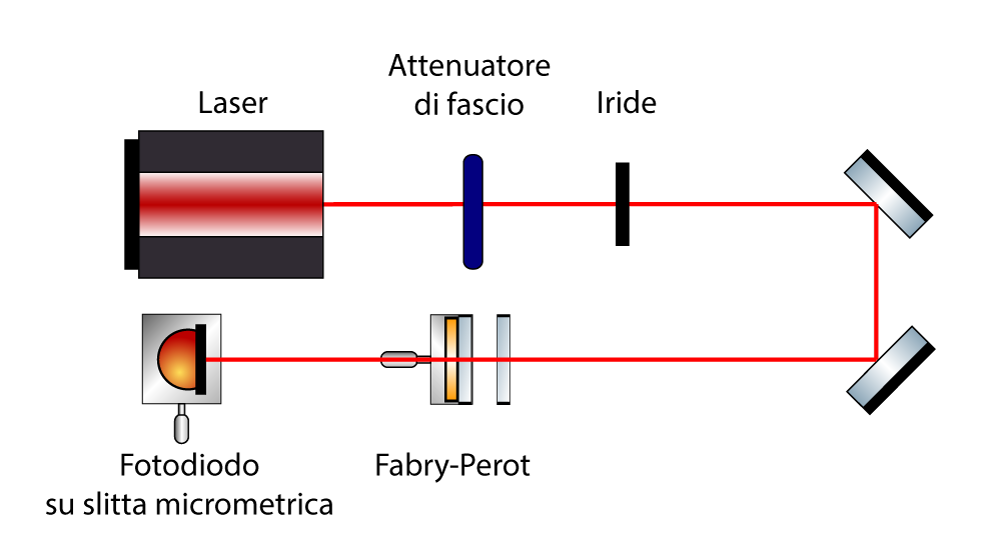
\includegraphics[width=1.1\linewidth]{diagram.png}}
	\captionof{figure}{Configurazione utilizzata.}
	\label{fig:diagram}
	\end{center}
\end{Figure}

Il segnale in uscita dal fotodiodo è inviato al \texttt{CH 2} dell'oscilloscopio \texttt{Tektronik TDS2012C}. Le misure di intensità luminosa vengono riportate come differenza di potenziale misurata ai capi del fotodiodo, pertanto è da intendere la presenza di un fattore di proporzionalità non noto. Inoltre, si regola con un filtro attenuatore l'intensità della luce emessa dal laser in modo da restare all'interno della regione di linearità del fotodiodo, ossia al di sotto di \SI{10}{V}. L'incertezza associata alle misure mediante i cursori è quella fornita dal manuale\footnote{\url{http://pdf1.alldatasheet.com/datasheet-pdf/view/554089/ETC2/TDS2012C.html}} dell'oscilloscopio, ossia il $3\%$.

Poiché il fotodiodo permette l'ingresso della luce attraverso un foro di diametro circa \SI{200}{\micro m}, si compiranno spostamenti della slitta micrometrica di almeno \SI{100}{\micro m}, e pertanto l'incertezza associata alla posizione del fotodiodo sarà di \SI{100}{\micro m}.

%==================================================
%             FIT DELLA FUNZIONE DI AIRY
%==================================================
\section{Misura della funzione di trasmissione e fit alla funzione di Airy}


%==================================================
%             MISURA DELLA FINESSE
%==================================================
\section{Misura della finesse al variare delle combinazioni di specchi}



%==================================================
%             MISURA DI LAMBDA
%==================================================
\section{Misura della lunghezza del Fabry-Perot e stima della lunghezza d'onda del laser}
Si verifica che per tutta la durata di questa presa dati il voltaggio del fotodiodo rimane compreso tra \SI{0}{} e \SI{0.6}{V}, dunque nella regione di linearità. Si rammenta che la distanza tra il fotodiodo e il secondo specchio del Fabry-Perot è $L=\SI{209 \pm 2}{mm}$; si interpone dunque tra il secondo specchio metallico e l'interferometro un foglio di plastica trasparente opaco quale mezzo diffusore, al fine di ottenere un'onda analoga a quella generata da una sorgente puntiforme. Oltre l'interferometro si osserva dunque il pattern di massimi e minimi circolari detto \emph{anelli di Airy}.

Si verifica che la posizione assoluta del secondo specchio dell'interferometro, rispetto allo zero della vite micrometrica che non necessariamente corrisponde alla distanza nulla tra gli specchi, è $d_1 = \SI{13.37 \pm 0.01}{mm}$.

Traslando la slitta su cui è posto il fotodiodo si misurano le posizioni di due massimi consecutivi e se ne stima l'angolo rispetto al centro del pattern come $\theta = (x-x_0) / L$. Si ha la relazione tra ordine del massimo e angolo 
\[
\frac{2d}{\lambda} \cos{\theta_m} = m
\]
sviluppando il coseno al secondo ordine si ottiene, dalla misura di due angoli,
\[
m \simeq \frac{2}{\theta_{m-1}^2 - \theta_{m}^2}
\]
e conoscendo il valore della lunghezza d'onda $\lambda$ (come dichiarato dal costruttore) si ottiene una stima della lunghezza del Fabry-Perot
\[
d \simeq \frac{m \lambda}{2},
\]
valida per $m \gg 1$.

Variando quindi la posizione assoluta del secondo specchio del Fabry-Perot, e portandolo a $d_2 = \SI{10.75 \pm 0.01}{mm}$, si ripete il procedimento precedente e si ricava l'ordine del massimo $m_2$. Quindi, si può stimare la lunghezza d'onda del laser da \[
\lambda^{\text{exp}} = \frac{2(d_1 - d_2)}{m_2 - m_1}.
\]

Si riportano in Tabella~\ref{tab:stimaLambda} i dati raccolti. La stima della lunghezza d'onda risulta essere
\[
\lambda^{\text{exp}} = \SI{633 \pm 14}{nm},
\]
compatibile con il valore fornito dal costruttore.

\begin{center}
\begin{table*}
\captionof{table}{Misure per la stima di $\lambda$}
\label{tab:stimaLambda}
\begin{tabular}{c|c|c|c|c|c}
 & $x_0$ [\SI{}{mm}] & $x_1$ [\SI{}{mm}] & $x_2$ [\SI{}{mm}] & $\theta_1$  & $\theta_2$ \\
 & $\pm 0.01$ & $\pm 0.1$ & $\pm 0.1$ & & \\
\hline 
$d_1 = \SI{13.37 \pm 0.01}{mm}$ & 10.70  & 12.7 & 11.8 &    \SI{9.6 \pm 1.0 e-3}{} & \SI{5.3 \pm 1.0 e-3}{} \\
$d_2 = \SI{10.75 \pm 0.01}{mm}$ & 14.8   & 13.1 & 8.4  & \SI{8.1 \pm 1.0 e-3}{} & \SI{31.0 \pm 1.0 e-3}{} \\
\hline
\end{tabular}
\begin{tabular}{c|c|c}
& m & d \\
\hline
$d_1 = \SI{13.37 \pm 0.01}{mm}$ & \SI{31.31 \pm 0.12 e3}{} & \SI{9.91 \pm 0.04}{mm}\\
$d_2 = \SI{10.75 \pm 0.01}{mm}$ & \SI{2.3 \pm 0.2 e3}{}  & \SI{0.73 \pm 0.06}{mm}\\
\hline
\end{tabular}
\end{table*}
\end{center}









\end{multicols}


\newpage
\section{Appendice}



%ESEMPIO DI FIGURA
%\begin{Figure}
%	\begin{center}
%	\includegraphics[width=\linewidth]{comune.png}
%	\captionof{figure}{Istantanea dell'oscilloscopio per l'amplificatore differenziale, misura di $A_c$}
%	\label{fig:Ac_differenziale}
%	\end{center}
%\end{Figure}


%ESEMPIO DI TABELLA
%\begin{center}
%\captionof{table}{Misure per la stima di $A_c$}
%\label{tab:Ac_differenziale}
%\begin{tabular}{c|c|c|c}
%$f$ [\SI{}{Hz}] & $V_i$ [\SI{}{V}] & $v_o$ [\SI{}{mV}] & $A_c = v_o / V_i$ \\
%\hline
%      149.5 &        3.90 &         11.3 & 2.90e-03 \\
%      222.0 &        3.90 &         11.5 & 2.95e-03 \\
%      281.0 &        3.90 &         11.8 & 3.03e-03 \\
%      359.0 &        3.90 &         11.8 & 3.03e-03 \\
%      461.0 &        3.90 &         12.2 & 3.13e-03 \\
%\hline
%\end{tabular}
%\end{center}


\end{document}
